% !TeX spellcheck = da_DK
\subsection{Forstærker i tilpasningsblok}
\subsubsection{Teori og design}
Jævnfør i afsnit \ref{Subsec:Forstaerker} på side \pageref{Subsec:Forstaerker} er der forklaret teorien samt designet af en forstærker, hvilket også gør sig gældende her. Da denne blok skal tilpasse det filtrerede signal til komparatoren, afgrænses måleintervallet til $\pm25^{\circ}$. Et range på $\pm90^{\circ}$ er unødvendigt ift. at vurdere hvorvidt patienten er faldet. Derfor ønskes det, at $V_{out}$ fra forstærkeren er $\pm5$V, når accelerometret måler $\pm25^{\circ}$. Denne forstærkning skal derved forstærke med en faktor 3, hvilket svarer til $9.5424$dB, som beskrevet i afsnit \ref{Tilpasningsblok} på side \pageref{Tilpasningsblok}. \\
For at udregne modstandene er R$2$ blevet valgt til $10$K$\Omega$. Ud fra dette er R$1$ blevet bestemt ved følgende udregning:
\begin{align}
3 = 1 + (\frac{R1}{10\text{K}\Omega})\\
R1 = 20\text{K}\Omega
\end{align}

\noindent Forstærkerens opbygning kan ses på \figref{fig:Forstaerker_faktor3}.
\begin{figure}[H]
	\centering
	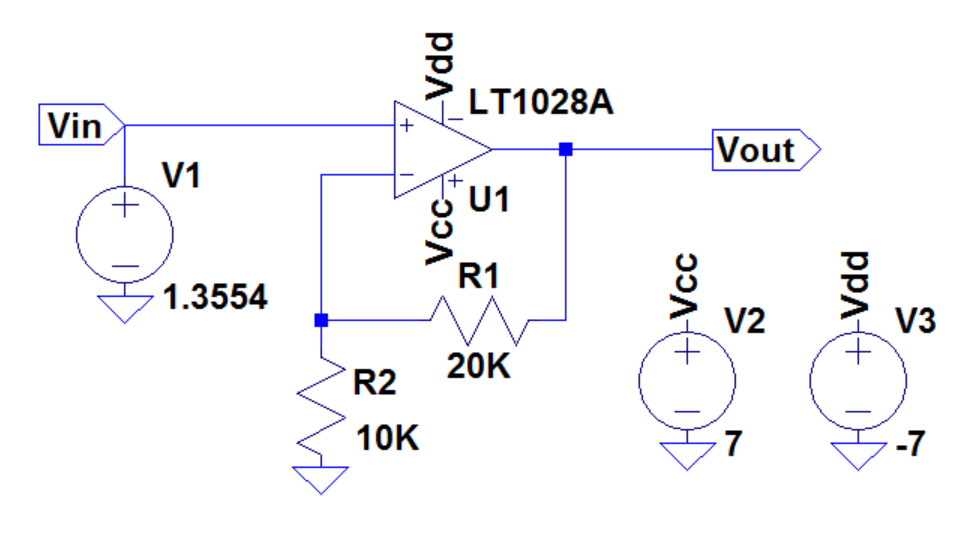
\includegraphics[scale=0.4]{figures/cProblemloesning/Forstaerker_faktor3.PNG}
	\caption{På figuren ses den ikke-inverterende opbygningen af forstærkeren, hvor der sker en forstærkning med en faktor $3$.}
	\label{fig:Forstaerker_faktor3}
\end{figure}

\subsubsection{Simulering}
Denne forstærker undersøges ligeledes i tre simuleringer for, hvorledes forstærkeren virker ved det laveste input , uden påvirkning samt højeste input. Det forstærkede signal, kaldet $V_{out}$, skal være $3$ gange større end $V_{in}$. Resultaterne af de fem simuleringer ses i \tableref{tab:forstarker3_simT}. Der er benyttet de teoretiske værdier, som er udregnet fra start.
\begin{table}[H]
	\centering
	\begin{tabular}{|l|l|l|l|l|}
		\hline
		\multicolumn{1}{|c|}{\textit{Inputsignalet} & \multicolumn{1}{c|}{\textit{Forstærkning}} & \multicolumn{1}{c|}{\textit{Forventet outputsignal}}                    & \multicolumn{1}{c|}{\textit{Outputsignalet}} & \multicolumn{1}{c|}{\textit{Afvigelse}} \\ \hline
		$4.8816$V     & 3   & \begin{tabular}[c]{@{}l@{}}Forventer mætning\\ $14.6448$V\end{tabular}  & $5.0530$V   & $\times$     \\ \hline
		$1.3554$V     & 3   & $4.0662$V                                                               & $4.0662$V   & $0\%$     \\ \hline
		$0$V          & 3   & $0$V                                                                    & $0$V        & $0\%$     \\ \hline
	   -$1.3302$V     & 3   & -$3.9906$V                                                              & -$3.9906$V  & $0\%$     \\ \hline
	   -$4.7880$V     & 3   & \begin{tabular}[c]{@{}l@{}}Forventer mætning\\ -$14.3640$V\end{tabular} & -$5.0527$V  & $\times$     \\ \hline
	\end{tabular}
		\caption{I tabellen ses resultaterne af de fem simuleringer.}
		\label{tab:forstarker3_simT}
\end{table}

Der ses, at der ingen afvigelse er. Kredsløbet fungere rent teoretisk med ideelle komponenter, som bliver brugt i LTspice. På \figref{Fig:simulering3faktor} ses simuleringen af $1.3554$V input, som ideelt vil komme fra filtret. På \figref{fig:faktor3_simulering}

\begin{figure}[H]
	\centering
	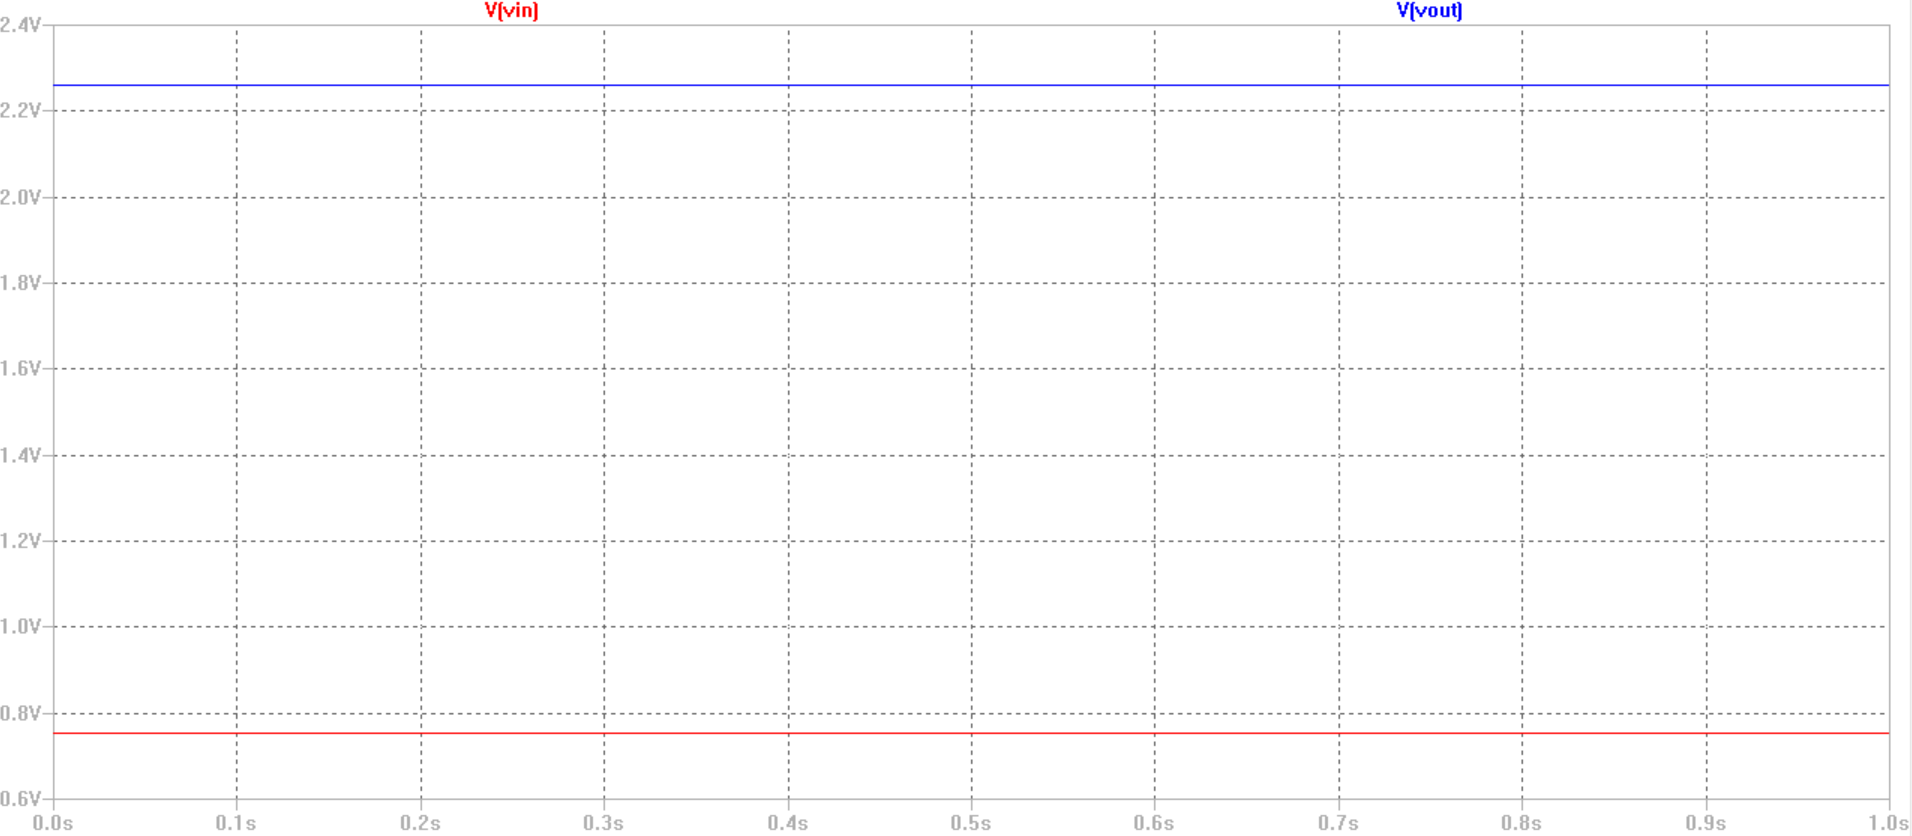
\includegraphics[scale=0.4]{figures/cProblemloesning/Forstaerker_faktor3_simulering.PNG}
	\caption{På figuren ses simuleringen af $1.3554$V input, som giver $4.0662$V i output. Der er altså sket en forstærkning med en faktor $3$.}
	\label{fig:faktor3_simulering}
\end{figure}

%\noindent Resultaterne af de fem simuleringer ses i \tableref{tab:forstarker3_simF}. Der er benyttet de værdier, som fås fra simuleringen med den første forstærker i afsnit \ref{Subsec:Forstaerker_simu} på side \pageref{Subsec:Forstaerker_simu}.
%\begin{table}[H]
%	\centering
%	\begin{tabular}{|l|l|l|l|l|}
%		\hline
%		\multicolumn{1}{|c|}{\textit{\begin{tabular}[c]{@{}c@{}}Simulerede\\ inputsignal\\ fra filter\end{tabular}}} & \multicolumn{1}{c|}{\textit{Forstærkning}} & \multicolumn{1}{c|}{\textit{Forventet outputsignal}}                      & \multicolumn{1}{c|}{\textit{Outputsignalet}} & \multicolumn{1}{c|}{\textit{Afvigelse}} \\ \hline
%		$4.8817$V   & 3    & \begin{tabular}[c]{@{}l@{}}Forventer mætning\\ (14,6451V)\end{tabular}    & XX  & XX   \\ \hline
%		$1.3560$V   & 3    & $4.0681$V                                                                 & XX  & XX   \\ \hline
%		$0$V        & 3    & $0$V                                                                      & XX  & XX   \\ \hline
%		-$1.3300$V  & 3    & -$3.9901$V                                                                & XX  & XX   \\ \hline
%		-$4.7881$V  & 3    & \begin{tabular}[c]{@{}l@{}}Forventer mætning\\ (-$14.3643$V)\end{tabular} & XX  & XX   \\ \hline
%	\end{tabular}
%		\caption{I tabellen ses resultaterne af de fem simuleringer.}
%		\label{tab:forstarker3_simF}
%\end{table}
\subsubsection{Implementering og test}